\documentclass[10pt,a4paper]{article}

\usepackage[utf8]{inputenc}
\usepackage[T1]{fontenc}
\usepackage[margin=2.0cm]{geometry}
\usepackage{graphicx}
\usepackage{booktabs}
\usepackage{amsmath}
\usepackage{subcaption}
\usepackage{caption}
\usepackage{xcolor}
\usepackage{enumitem}
\usepackage{tikz}
\usetikzlibrary{arrows.meta,positioning,shapes.geometric}
\usepackage[colorlinks=true,linkcolor=blue!50!black,urlcolor=blue!50!black]{hyperref}

\setlist{nosep,leftmargin=*}
\captionsetup{font=small,labelfont=bf}
\setlength{\parindent}{0pt}
\setlength{\parskip}{3pt}
\setlength{\abovecaptionskip}{3pt}
\setlength{\belowcaptionskip}{0pt}
\setlength{\floatsep}{8pt plus 2pt minus 2pt}
\setlength{\textfloatsep}{8pt plus 2pt minus 2pt}

% Placeholder for everything that still has to be filled in after the final run.
% Search for "TBD" in this file before submitting.
\newcommand{\tbd}[1]{\textbf{\textcolor{red!70!black}{[TBD: #1]}}}
\newcommand{\tbdc}{\textbf{\textcolor{red!70!black}{TBD}}}

\title{\vspace{-1.2cm}\textbf{Assessing Bicycle Lane Quality Using Smartphone Sensor Data}\\[2pt]
\large 5ARE0 -- Assignment 1}
\author{Group 41\\
\small \tbd{names and student numbers of the three members}}
\date{\small October 2026}

\begin{document}
\maketitle
\vspace{-0.8cm}


%=====================================================================
\section{Business and Objective Understanding}
%=====================================================================

Cycling is only as safe and comfortable as the lane it happens on. Cracks, potholes, root bumps and raised joints make a ride tiring, they push the rider into sudden corrections, and they increase the risk of falls. At the same time, cities cannot afford to inspect every kilometre of bike lane by hand. Everyone who rides already carries a phone with an accelerometer, a gyroscope and a gravity sensor, so the idea is to let the rides themselves do the inspection.

Our objective is a binary classifier that, given a short time window of phone sensor data recorded on a bike, says whether the lane under the wheels is \emph{smooth} or \emph{bumpy}. From the health and monitoring side, this is a cheap proxy for the vibration a rider is exposed to and for the places where a lane is likely to cause discomfort or accidents. From the city side, it is a way to rank lanes for maintenance.

We define success as follows, before looking at any result:
\begin{itemize}
  \item \textbf{Main metric:} macro-averaged F1 on recordings the model has never seen (not on windows from recordings it has seen), because the classes are unbalanced (6 vs.\ 9 recordings) and a ``bumpy'' lane that is missed matters as much as a false alarm.
  \item \textbf{Secondary:} per-class precision and recall, confusion matrices, and for the unsupervised models the Adjusted Rand Index (ARI).
  \item \textbf{Practical:} the final model has to run on a phone, so it must work with a small feature set and negligible inference cost, and it has to work on an external dataset we do not control (Section~\ref{sec:deploy}).
\end{itemize}

%=====================================================================
\section{Data Understanding}
%=====================================================================

\subsection{Collection methodology}

We recorded with the free \emph{Sensor Logger} app, with only the accelerometer, gyroscope and gravity sensors enabled, the default 100~Hz sampling rate, and the \emph{Standardisation} option on so that iOS and Android data are comparable. A recording starts with the screen tap on the phone, the rider cycles along one lane, and the recording stops with another tap.

\textbf{Placement.} The assignment suggests a pocket, an armband or a waistband. We chose none of them. We fixed the phone \emph{vertically on the straight part of the handlebar}, screen facing the rider, using a bike phone support. The reasoning is that a pocket or a waistband mixes the road signal with leg movement and pedalling, and the phone moves relative to the body. A rigid handlebar mount sees the road through the front wheel and the fork, and it moves with the bike, so what is left is mostly the motion of the bike on the surface. The price is that the support is not identical across bikes: the tilt of the holder changes from one bike (and one session) to another, which is why we need the alignment step in Section~\ref{sec:align}. 


\textbf{Dataset.} We have 15 recordings in and around Eindhoven (campus roads, the station area, the stadium area, residential streets), collected in September 2026  by 2 riders on 2 iphones. Each recording was labelled \emph{at recording time} as smooth or bumpy by the rider: smooth means a regular red cycling lane without imperfections, bumpy means a lane with visible rough features (potholes, cracks, raised joints, uneven surface) that is still safe to ride. The label lives in the recording name. 

\subsection{Exploratory analysis}

\textbf{Mounting differs a lot between recordings.} From the median gravity vector of each recording we estimated the pitch $\theta$ of the holder around the handlebar and the roll $\psi$ of the phone inside the holder (Table~\ref{tab:rec}). The pitch goes from about $0^\circ$ to $-40^\circ$. Without correcting for this, the same bump would show up on different axes in different recordings, and any axis-wise feature would mostly measure the holder, not the road. In the raw gravity of Figure~\ref{fig:align}, one recording has $g_y\approx-8$ and $g_z\approx-5.7$ m/s$^2$ instead of $(0,-9.8,0)$.

\begin{table}[!htbp]
\centering
\caption{The 15 recordings with the mounting angles estimated from the median gravity, and quality checks of the alignment. All recordings have median $|g|$ between 9.798 and 9.806~m/s$^2$ and no warning was raised.}
\label{tab:rec}
\scriptsize
\begin{tabular}{llrrrr}
\toprule
Recording & Class & Pitch $\theta$ [$^\circ$] & Roll $\psi$ [$^\circ$] & Drift [$^\circ$] & Residual [$^\circ$]\\
\midrule
\texttt{bumpy\_con\_tante\_buche} & bumpy & 0.28 & 2.13 & 1.00 & 0.001\\
\texttt{bumpy\_con\_una\_grande\_curva\_alla\_fine} & bumpy & $-13.12$ & 3.24 & 0.90 & 0.015\\
\texttt{bumpy\_stadio} & bumpy & $-35.41$ & 4.18 & 1.98 & 0.008\\
\texttt{bumpy\_stazione} & bumpy & $-35.02$ & 3.25 & 0.70 & 0.003\\
\texttt{bumpy\_stradabumpy\_con\_rialzi\_e\_buche} & bumpy & $-14.39$ & 2.68 & 0.54 & 0.004\\
\texttt{bumpy\_swapfiets} & bumpy & $-34.27$ & 3.76 & 1.67 & 0.040\\
\texttt{smooth\_con\_fermata} & smooth & $-24.95$ & 2.52 & 1.15 & 0.005\\
\texttt{smooth\_con\_fermata\_2} & smooth & $-24.99$ & 2.32 & 1.80 & 0.005\\
\texttt{smooth\_con\_un\_po\_di\_rialzi\_e\_piccoli\_tratti\_\dots} & smooth & 0.79 & 2.86 & 1.75 & 0.001\\
\texttt{smooth\_grande\_curva\_apl\_inizio} & smooth & 0.17 & 2.41 & 1.76 & 0.001\\
\texttt{smooth\_ma\_con\_irregolarita\_periodiche\_foto} & smooth & $-13.97$ & 2.41 & 0.63 & 0.011\\
\texttt{smooth\_monknatlab} & smooth & $-35.26$ & 4.69 & 0.18 & 0.015\\
\texttt{smooth\_quartiere\_bene\_eindhoven} & smooth & $-34.48$ & 2.87 & 0.39 & 0.011\\
\texttt{smooth\_strada\_universiya\_ingresso} & smooth & 0.51 & 2.98 & 0.61 & 0.000\\
\texttt{smooth\_strda\_turca} & smooth & $-40.04$ & 3.00 & 1.53 & 0.007\\
\bottomrule
\end{tabular}
\end{table}

\textbf{Frequency content.} Before designing any filter we looked at the spectra of the aligned signals: the whole-signal FFT, the Welch power spectral density and the spectrogram. The main findings:
\begin{itemize}
  \item \emph{Accelerometer.} Bumpy and smooth PSDs separate clearly above about 20~Hz on all three axes (Figure~\ref{fig:psd}a), and on the Y (vertical) and Z axes the bumpy median shows an extra peak near 14~Hz, although its spread is large. Both classes share a baseline around 10--20~Hz (rolling, pedalling, frame resonance): the \emph{amount} of vibration discriminates, not its presence.
  \item \emph{Gyroscope.} The separation is clearest on the X axis from about 5~Hz up; on Y and Z it is small. Below roughly 5~Hz the gyroscope is dominated by steering and leaning, which has nothing to do with the surface.
  \item \emph{Spectrogram.} The bumpy spectrograms show a sustained elevated band instead of isolated vertical streaks (Figure~\ref{fig:spec}). Our bumpy recordings therefore capture continuous roughness more than isolated potholes; we have not verified this with a recording of single, well-separated potholes.
  \item Above $\sim$40~Hz (close to Nyquist) the classes still diverge, but we treat this as sensor noise and leave it out of the band.
\end{itemize}

\begin{figure}[!htbp]
\centering
\begin{subfigure}[t]{0.49\linewidth}
  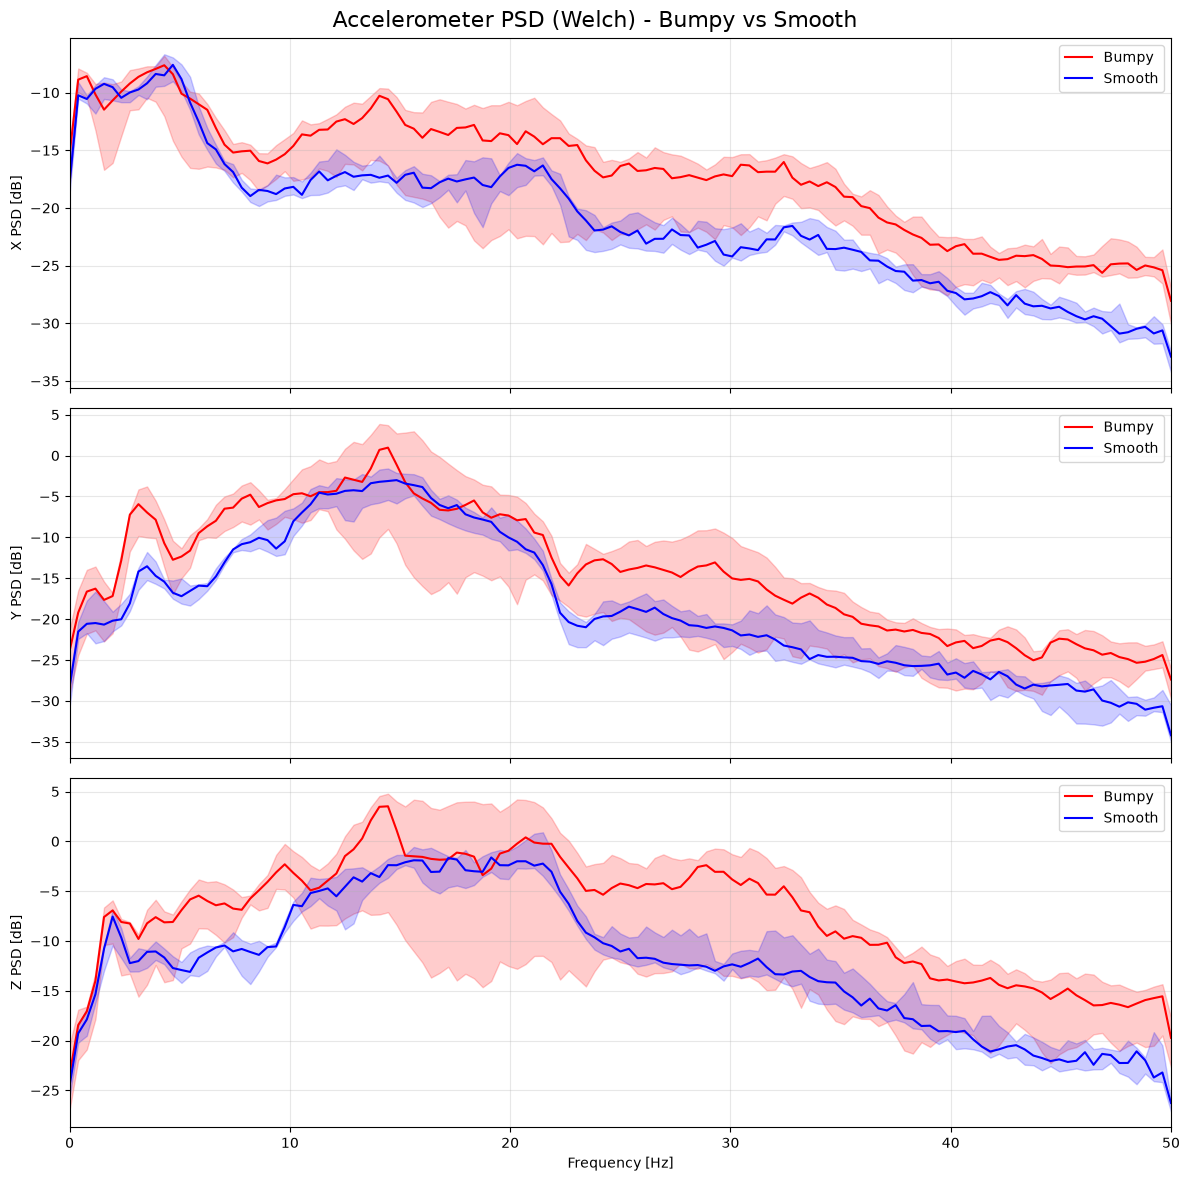
\includegraphics[width=\linewidth]{psd_acc.png}
  \caption{Accelerometer}
\end{subfigure}\hfill
\begin{subfigure}[t]{0.49\linewidth}
  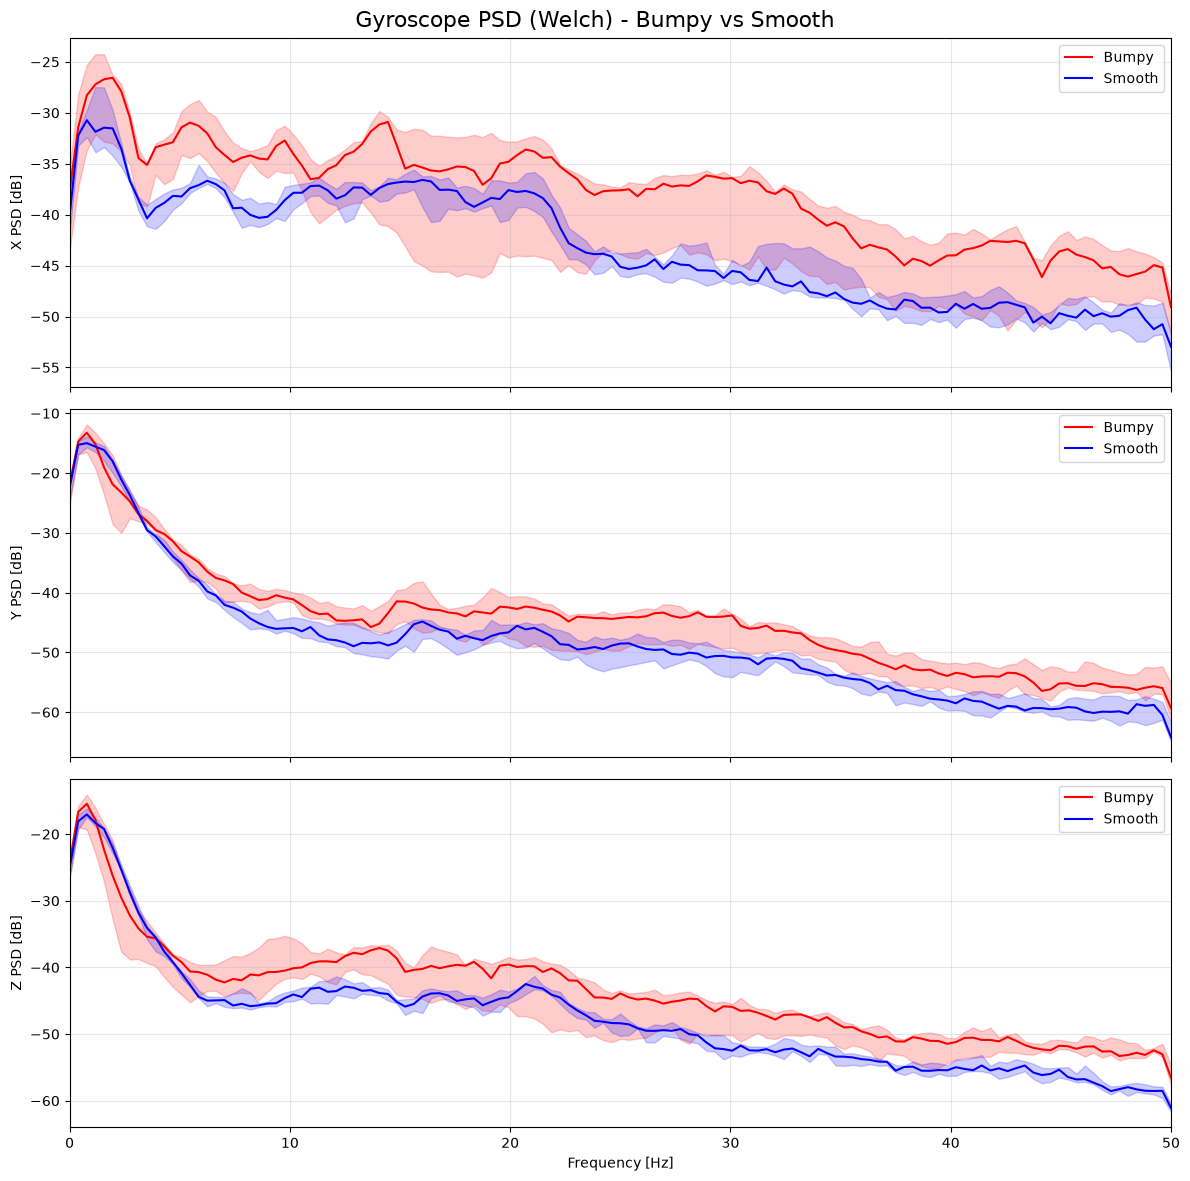
\includegraphics[width=\linewidth]{psd_gyr.png}
  \caption{Gyroscope}
\end{subfigure}
\caption{Welch PSD of the aligned signals, median and inter-quartile range over the 6 bumpy (red) and 9 smooth (blue) recordings.}
\label{fig:psd}
\end{figure}

\begin{figure}[!htbp]
\centering
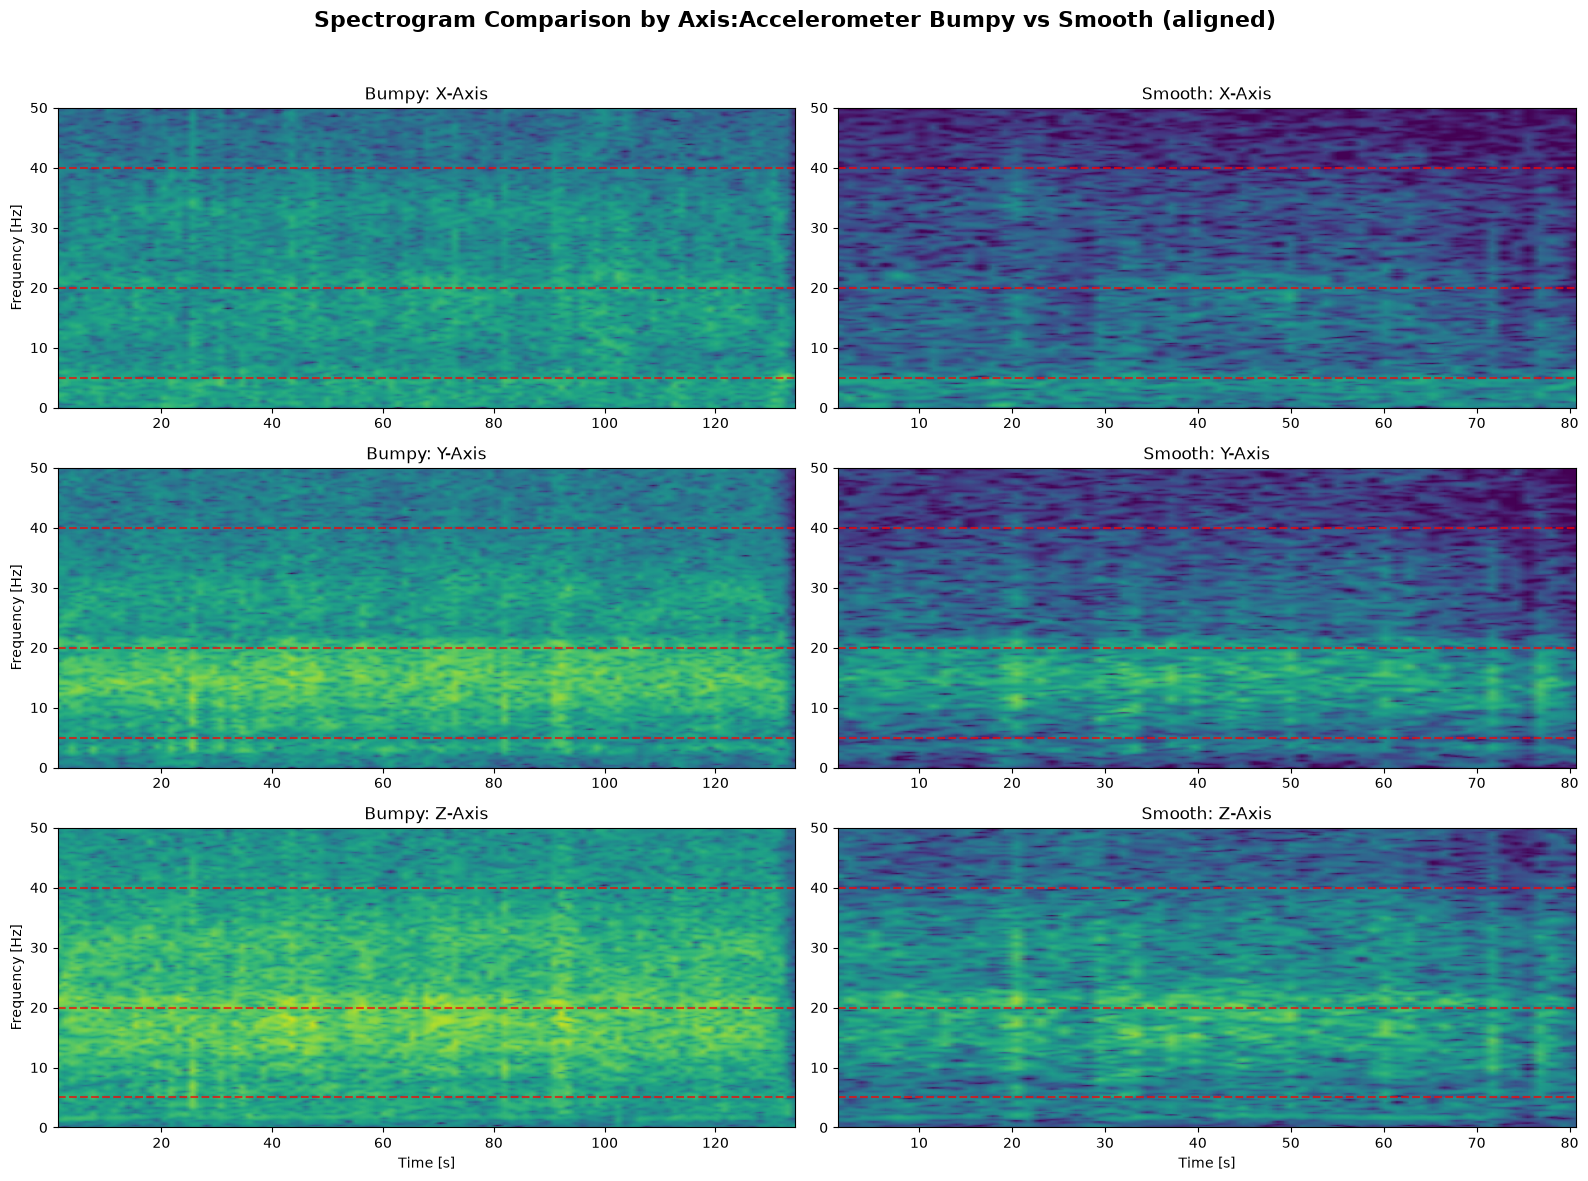
\includegraphics[width=0.62\linewidth]{spectrogram_acc.png}
\caption{Accelerometer spectrograms (aligned) of one bumpy and one smooth recording on the same axes. Dashed lines mark 5, 20 and 40~Hz.}
\label{fig:spec}
\end{figure}

\subsection{Data quality and limitations}
\label{sec:quality}

\begin{itemize}
  \item \textbf{Synchronisation.} The three sensors of a recording may differ by at most 5 samples in length (otherwise the notebook stops); they are truncated to the shortest.
  \item \textbf{Alignment quality.} After alignment the median gravity is within 0.04$^\circ$ of $(0,-g,0)$ for every recording, and the angle between the median gravity of the first and last 20\% of each recording is at most 1.98$^\circ$ (threshold 5$^\circ$), i.e.\ the phone did not move in its holder.
  \item \textbf{Very small dataset.} 15 recordings is little. Windows overlap and come from the same ride, so they are strongly correlated: 630 windows are far fewer than 630 independent samples. This is why every split in this work is grouped by recording.
  \item \textbf{Class and session confounding.} The mounting pitch clusters by session (Table~\ref{tab:rec}): the two recordings at $\approx-25^\circ$ are both smooth, the four at $\approx 0^\circ$ are three smooth and one bumpy, the five at $\approx-35^\circ$ are three bumpy and two smooth. A classifier could pick up differences of bike, phone, rider or tyre instead of road quality, and with groups defined as single recordings we cannot rule this out. Speed was not recorded either, although vibration amplitude grows with speed.
  \item \textbf{Label noise.} Labels are one per recording, assigned from our judgement. A recording called ``smooth with a few raised bits and small jumpy sections'' still carries the label smooth for all its windows.
  \item \textbf{No GPS.} We cannot correct for slope or steering, and we cannot place results on a map for our own data.
\end{itemize}

%=====================================================================
\section{Data Preparation}
%=====================================================================

\begin{figure}[!htbp]
\centering
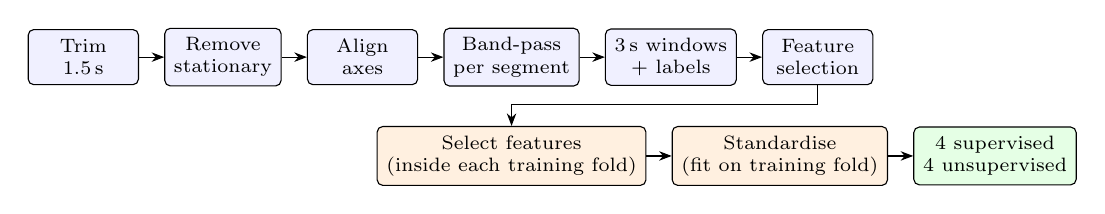
\begin{tikzpicture}[node distance=3.0mm and 3.2mm, every node/.style={font=\scriptsize},
  box/.style={draw,rounded corners=2pt,minimum height=7mm,minimum width=14mm,align=center,fill=blue!6},
  arr/.style={-{Stealth[length=1.6mm]}}]
  \node[box] (a) {Trim\\1.5\,s};
  \node[box,right=of a] (b) {Remove\\stationary};
  \node[box,right=of b] (c) {Align\\axes};
  \node[box,right=of c] (d) {Band-pass\\per segment};
  \node[box,right=of d] (e) {3\,s windows\\+ labels};
  \node[box,right=of e] (f) {Feature\\selection};
  \draw[arr] (a)--(b); \draw[arr] (b)--(c); \draw[arr] (c)--(d); \draw[arr] (d)--(e); \draw[arr] (e)--(f);
  \node[box,fill=orange!12,below=5mm of d] (g) {Select features\\(inside each training fold)};
  \node[box,fill=orange!12,right=of g] (h) {Standardise\\(fit on training fold)};
  \node[box,fill=green!10,right=of h] (i) {4 supervised\\4 unsupervised};
  \draw[arr] (f.south) -- ++(0,-2.5mm) -| (g.north);
  \draw[arr] (g)--(h); \draw[arr] (h)--(i);
\end{tikzpicture}
\caption{Pipeline. Blue steps use no labels and no information from other recordings, orange steps are fitted only on the training folds of the cross-validation.}
\label{fig:pipe}
\end{figure}

\subsection{Preprocessing pipeline and rationale}

\textbf{1. Sign convention.} iOS and Android report accelerometer and gravity with opposite signs (inertial vs.\ applied force); the gyroscope has the same sign on both. We convert everything to the iOS convention, using the recording metadata (platform and standardisation flag) and, if that is missing, the sign of the gravity $y$ component. With this convention a bike at rest on flat ground has gravity $\approx(0,-9.81,0)$.

\textbf{2. Trimming.} The first and last 1.5\,s (150 samples) of every recording are cut. They contain the taps on the screen.

\textbf{3. Stationary segments.} A stop at a traffic light says nothing about the lane. We compute the squared accelerometer magnitude, average it over a rolling window of 50 samples (0.5\,s), and mark a sample as stationary if this energy is below 0.30 (m/s$^2)^2$. Only runs of at least 200 samples (2\,s) are removed, so short pauses in a ride survive. The removal leaves time gaps, so later steps that depend on continuity (filtering, windowing) are done per continuous segment: 15 recordings become 18 segments.

\begin{figure}[!htbp]
\centering
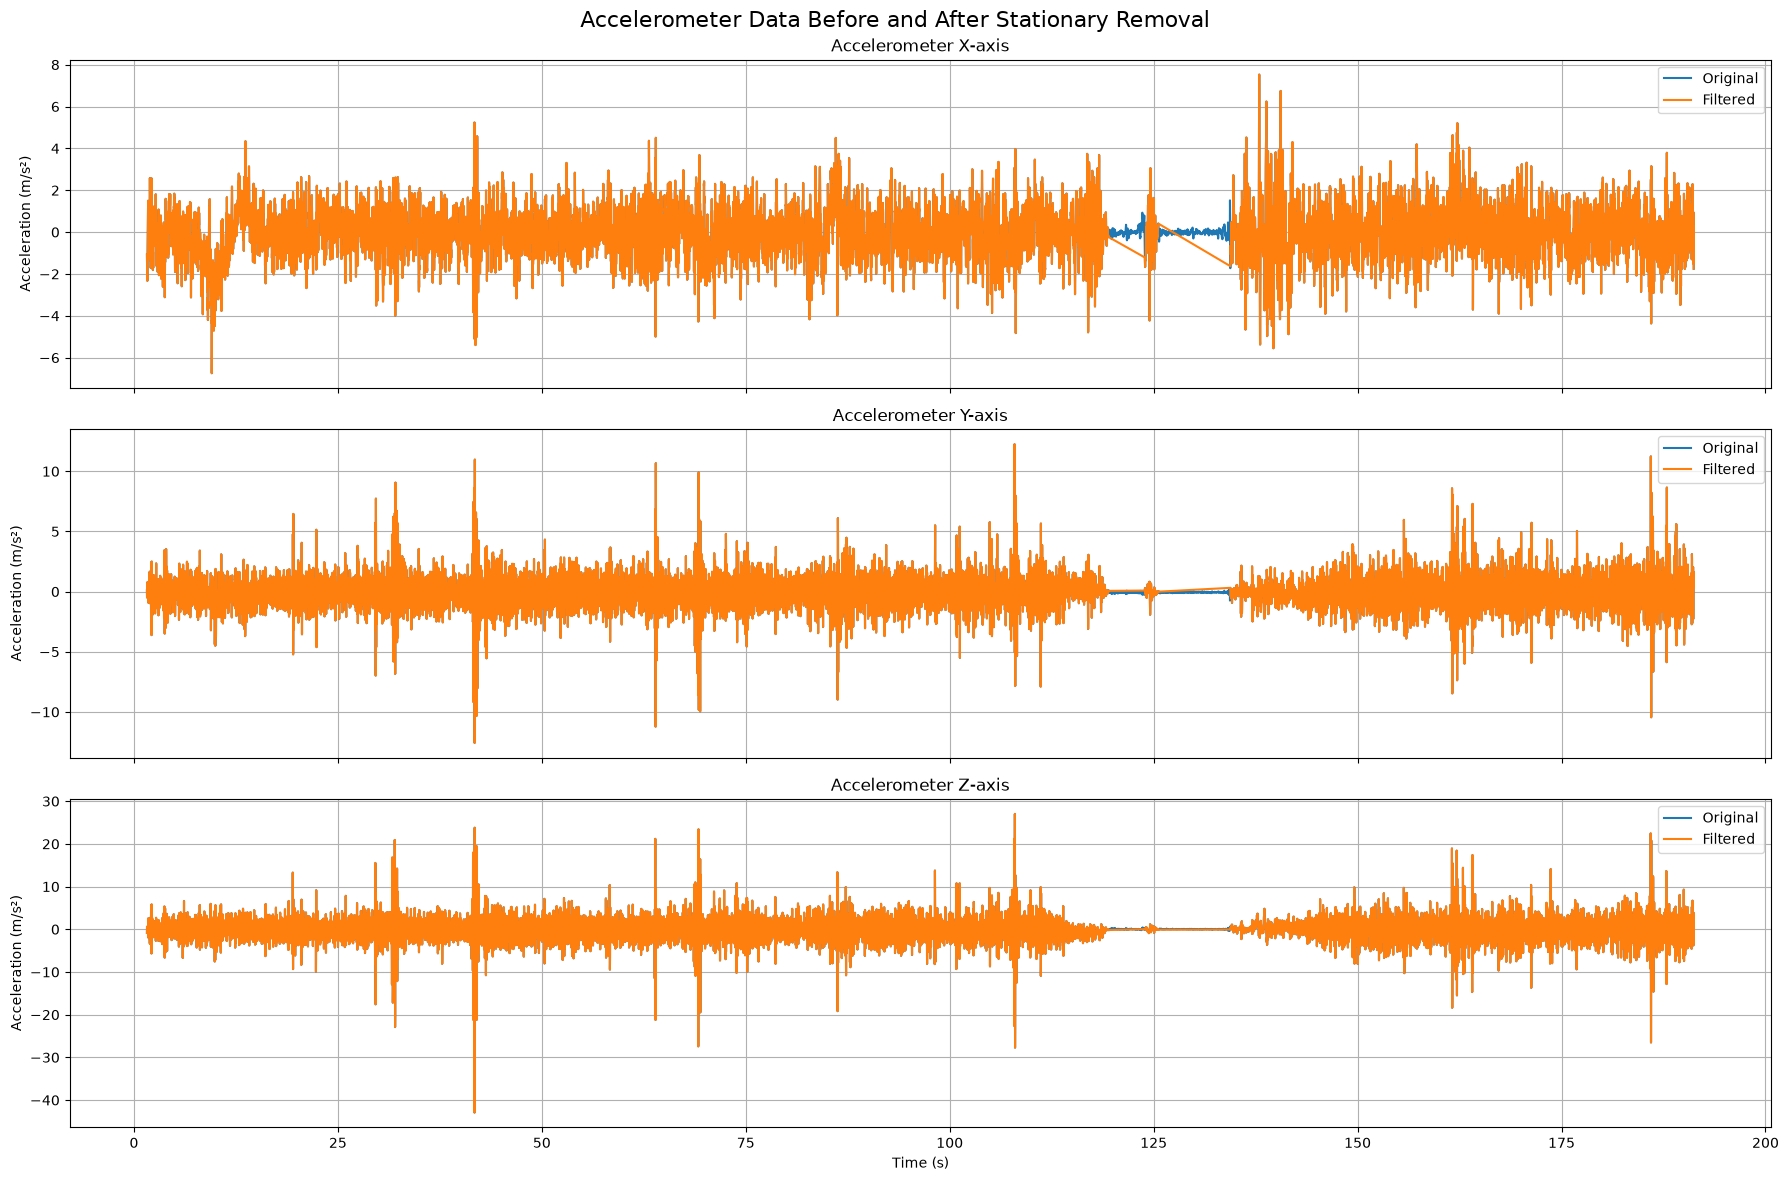
\includegraphics[width=0.52\linewidth]{stationary_removal.png}
\caption{Accelerometer of \texttt{smooth\_con\_fermata} before (blue) and after (orange) stationary removal. The straight line is only the plot joining the two sides of the removed stop.}
\label{fig:stat}
\end{figure}

\textbf{4. Axis alignment.}\label{sec:align} We want every recording expressed in the same \emph{bike frame}: $x$ along the handlebar towards the rider's left, $y$ perpendicular to the road (down), $z$ in the travel direction. The holder has two degrees of freedom, a roll $\psi$ of the phone around its screen normal and a pitch $\theta$ of the holder around the handlebar. With $u=-g_{\mathrm{med}}/\|g_{\mathrm{med}}\|$ the unit vector pointing up, in the phone axes (and $g_{\mathrm{med}}$ the component-wise median gravity of the whole recording, which is robust to curves, bumps and braking):
\begin{equation}
u=(\cos\theta\sin\psi,\ \cos\theta\cos\psi,\ -\sin\theta),\qquad
\psi=\operatorname{atan2}(u_x,u_y),\quad \theta=\operatorname{atan2}\!\left(-u_z,\sqrt{u_x^2+u_y^2}\right).
\end{equation}
One constant rotation $R=R_x(\theta)R_z(\psi)$ per recording is then applied to every sample of the accelerometer, gyroscope and gravity: $v'=R\,v$, which gives $R\,g_{\mathrm{med}}=(0,-\|g\|,0)$.


\begin{figure}[!htbp]
\centering
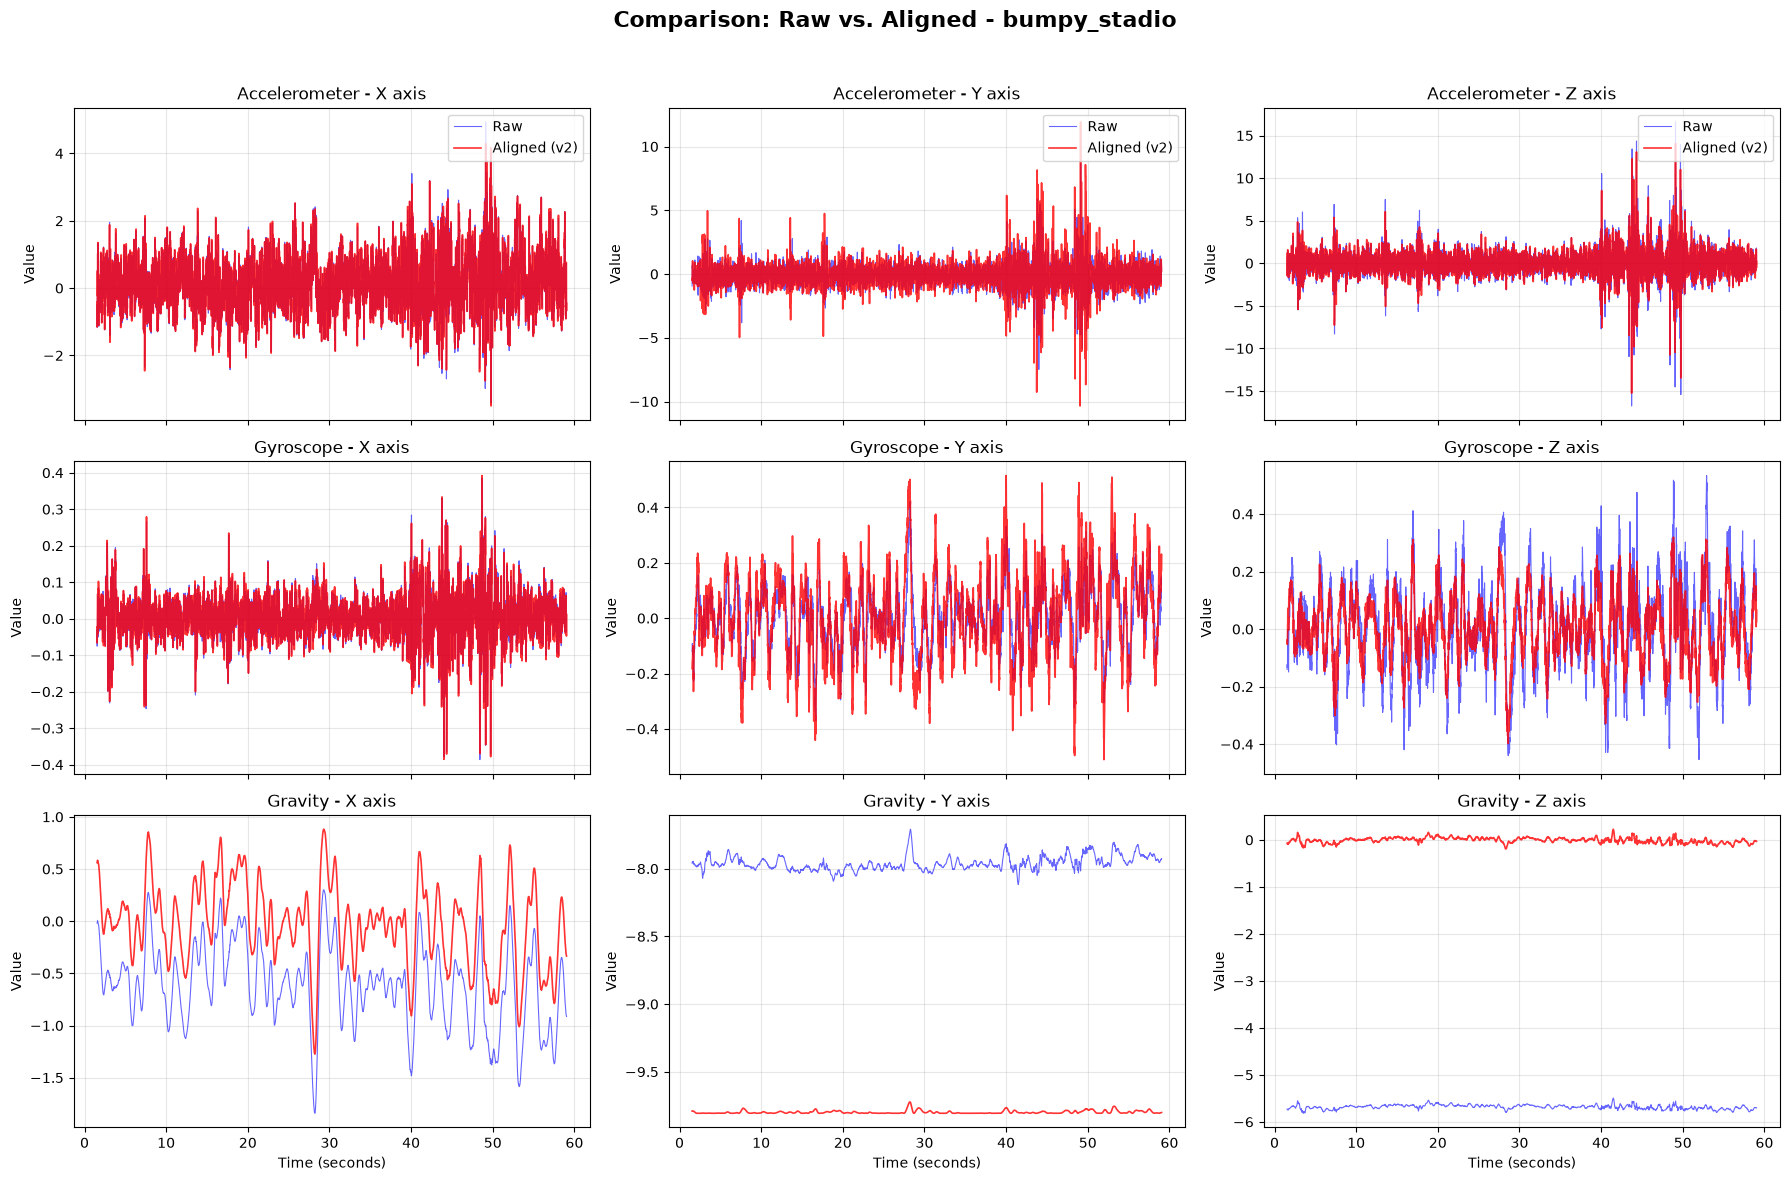
\includegraphics[width=0.68\linewidth]{alignment.png}
\caption{\texttt{bumpy\_stadio}, raw (blue) vs.\ aligned (red). Accelerometer and gyroscope keep their dynamics but move between axes; the gravity components are what the alignment is built on (the aligned gravity is a constant $(0,-9.8,0)$).}
\label{fig:align}
\end{figure}

\textbf{5. Band-pass filter.} The filter band comes from the spectral analysis above, balancing the statistical separation with physical constraints. We use a 4th-order Butterworth band-pass applied forwards and backwards (\texttt{filtfilt}, zero phase) with \textbf{10--40~Hz for the accelerometer} and \textbf{5--40~Hz for the gyroscope}. The upper edge drops the region close to Nyquist, where we suspect sensor noise. The lower edges drop gravity residuals, pedalling and, for the gyroscope, the steering and leaning below 5~Hz. For the accelerometer, the PSD clear separation lives above $\sim$20~Hz, but the main physical impact of a wheel on a pothole is expected around 10--15~Hz, so we kept the range from 10~Hz. The filter is applied to each continuous segment separately (gap larger than 0.2\,s starts a new segment; segments shorter than 0.5\,s are dropped), otherwise the jumps created by stationary removal would leak broadband energy into the filtered signal. One thing worth to notice: the band was chosen by looking at all 15 recordings, so it is not fully independent of the test recordings in the cross-validation. The band is wide, label-free in its application and only inspected visually, so we consider the leakage very small.

\textbf{6. Windowing and labels.} We cut 3\,s windows with 30\% overlap, only inside a continuous segment, and each window inherits the label of its recording (bumpy = 1, smooth = 0). Three seconds contain many periods even of the lowest passband frequency and give a Welch resolution of 0.67~Hz, enough to resolve bands of 5--10~Hz; overlap increases the number of windows and prevents a single bump from being cut in half by a window boundary. We chose these values a priori and did not run a sensitivity study on the window length. The result is \textbf{630 windows}, each carrying its recording as a group identifier.

\subsection{Feature engineering, extraction and selection}

Each window is described by features computed on each of the six channels (accelerometer and gyroscope, X/Y/Z), always on the band-passed signal.
\begin{itemize}
  \item \textbf{Time domain (8):} mean, standard deviation, RMS, maximum, minimum, peak-to-peak, energy, and peak count.
  \item \textbf{Frequency domain (6):} dominant frequency, spectral centroid, spectral entropy, spectral flatness, geometric mean and arithmetic mean of the normalised PSD (Welch with 150-sample segments, restricted to the passband of the sensor).
  \item \textbf{Band energies:} accelerometer 10--20, 20--30, 30--40~Hz; gyroscope 5--10, 10--20, 20--30, 30--40~Hz.
\end{itemize}
This gives $3\cdot17+3\cdot18=\mathbf{105}$ features per window. Many of them are redundant \emph{by construction}: after band-passing, the mean is $\approx0$, so standard deviation, RMS and energy are practically the same quantity; the arithmetic mean of a normalised PSD is just $1/N_{\mathrm{bins}}$ (a constant, mutual information 0); and the geometric mean and flatness differ by that constant. The peak count with a $0.5\sigma$ threshold yields about 100 peaks per 300 samples even on smooth lanes, so it behaves more like a noise-density measure than a count of impacts, which agrees with its low mutual information. The selection step below is what deals with this.

\textbf{Selection is different for supervised and unsupervised models, on purpose.} If we reused the supervised features for clustering, we would hand the clustering algorithms features chosen to separate the labels, and the ARI would be inflated. Fisher-score type criteria need the labels too. So:
\begin{itemize}
  \item \textbf{Supervised} (one feature set per model and per outer fold, computed only on the outer training set): \newline 
  (i) rank all features by mutual information with the label; \\
  (ii) compute the correlation matrix and drop any feature with $|\rho|>0.8$, keeping most informative feature with respect to the label between the two; \\
  (iii) forward selection on the survivors in rank order, adding a feature only if it improves the macro-F1 of \emph{that model} by more than 0.01 in an inner 3-fold grouped cross-validation (the first four are always taken, at most 12 are kept). The scaler is fitted inside each inner fold. \\
  \item \textbf{Unsupervised} (no labels at all): drop features with $|\rho|>0.9$ to an earlier one, standardise, and project with PCA on the training fold, keeping at most 6 components. The 85\% variance target is never reached, the 6 components cap explains 61--64\% of the variance in all five folds, so that cap is what decides.
\end{itemize}
\\

\textbf{Normalisation.} Features are standardised ($z$-score) with a \texttt{StandardScaler} fitted on the training portion only and applied unchanged to the test portion, inside every fold. This is required for KNN, SVM and logistic regression (distance- and margin-based), it is harmless for Random Forest, and for PCA it is needed to prevent high-variance features such as energies from dominating.

%=====================================================================
\section{Modeling}
%=====================================================================

\textbf{Validation scheme.} Outer 5-fold \texttt{GroupKFold} with the recording as group: the 15 recordings are split into five folds, and no recording ever contributes windows to both training and test. A random window-level split would put almost identical neighbouring windows on both train and test sides, causing data leakage and accuracies above what a new ride would get. Feature selection, scaling and PCA are re-fitted on the training part of every fold, and the test fold is touched only for the final prediction. 

\textbf{Supervised models.} We chose four models that cover different assumptions: \\ \textbf{K-Nearest Neighbours} ($k=5$, local, non-parametric),\\  \textbf{Logistic Regression} (linear baseline, interpretable weights),\\  \textbf{Random Forest} (100 trees, non-linear, robust to feature scale), \\ \textbf{SVM} (RBF kernel). Each one gets its own feature subset from the procedure above.

\textbf{Unsupervised models.} \textbf{K-Means}, \textbf{agglomerative (hierarchical) clustering}, \textbf{Gaussian Mixture Model} and \textbf{DBSCAN}, all on the 6 PCA components. K-Means, hierarchical and GMM are run with 2 clusters, to compare with the two classes. DBSCAN does not need the number of clusters; its $\varepsilon$ and minimum number of points are \tbd{how chosen, e.g.\ k-distance plot}. Clusters are compared with the labels only afterwards, through ARI, normalised mutual information, silhouette, and, for a confusion matrix, by mapping each cluster to the majority class. Held-out windows are assigned to the clusters fitted on the training windows (\tbd{assignment rule for held-out windows, in particular for DBSCAN and hierarchical}).

\textbf{Comparison methodology.} All eight models see the same outer folds. Supervised models are scored by (\tbd{macro-F1, accuracy and per-class recall; unsupervised ones by ARI and by the macro-F1 after the majority-class mapping, so that the two families can be put side by side. We report the mean and the standard deviation over folds, plus the pooled confusion matrix over all test folds. Because a test fold contains only three recordings, differences of a few points between models are not significant, and we do not claim a winner on them.}

%=====================================================================
\section{Evaluation}
%=====================================================================

\subsection{Performance metrics and results}

\begin{table}[!htbp]
\centering
\caption{Test performance, mean $\pm$ standard deviation over the 5 outer folds (each test fold = 3 unseen recordings). Unsupervised models: majority-class mapping for F1/accuracy.}
\label{tab:res}
\small
\begin{tabular}{lccccc}
\toprule
Model & Macro-F1 & Accuracy & Recall bumpy & Recall smooth & ARI\\
\midrule
KNN ($k=5$)              & \tbdc & \tbdc & \tbdc & \tbdc & --\\
Logistic Regression      & \tbdc & \tbdc & \tbdc & \tbdc & --\\
Random Forest            & \tbdc & \tbdc & \tbdc & \tbdc & --\\
SVM (RBF)                & \tbdc & \tbdc & \tbdc & \tbdc & --\\
\midrule
K-Means                  & \tbdc & \tbdc & \tbdc & \tbdc & \tbdc\\
Hierarchical             & \tbdc & \tbdc & \tbdc & \tbdc & \tbdc\\
GMM                      & \tbdc & \tbdc & \tbdc & \tbdc & \tbdc\\
DBSCAN                   & \tbdc & \tbdc & \tbdc & \tbdc & \tbdc\\
\bottomrule
\end{tabular}
\end{table}

During feature selection every candidate subset was scored with the macro-F1 of an inner 3-fold grouped cross-validation on the training recordings (Table~\ref{tab:inner}). These are \emph{not} test results: the subset is chosen to maximise this number, so it is optimistically biased. They are still informative about two things. First, the scores are modest and swing a lot between outer folds (0.53 to 0.90): which recordings end up in training matters more than which of the four classifiers is used. Second, the four classifiers are within the fold-to-fold spread of each other, so with this much data we expect their test scores to be hard to tell apart as well. \tbd{replace/extend with the final test results once training is done}

\begin{table}[!htbp]
\centering
\caption{Best inner-CV macro-F1 reached by the forward selection, per model and outer fold (selection-time score, optimistically biased, not a test result).}
\label{tab:inner}
\small
\begin{tabular}{lcccccc}
\toprule
Model & Fold 1 & Fold 2 & Fold 3 & Fold 4 & Fold 5 & Mean $\pm$ std\\
\midrule
KNN                 & 0.882 & 0.732 & 0.727 & 0.647 & 0.793 & 0.756 $\pm$ 0.078\\
Logistic Regression & 0.902 & 0.693 & 0.691 & 0.548 & 0.753 & 0.717 $\pm$ 0.114\\
Random Forest       & 0.837 & 0.715 & 0.693 & 0.620 & 0.773 & 0.728 $\pm$ 0.073\\
SVM                 & 0.874 & 0.732 & 0.622 & 0.528 & 0.797 & 0.711 $\pm$ 0.123\\
\bottomrule
\end{tabular}
\end{table}

\subsection{Selected features}

Across the 20 selections (4 models $\times$ 5 folds) the chosen subsets have 4 to 9 features. They agree strongly within a fold (the mutual-information ranking and the correlation filter decide most of the choice) and much less across folds, which is a sign of how unstable selection is with 12 training recordings. The most stable features are:

\begin{table}[!htbp]
\centering
\caption{Features most often selected (out of 20 selections, 4 models $\times$ 5 folds).}
\label{tab:feat}
\small
\begin{tabular}{lcc}
\toprule
Feature & Selections & Folds (of 5)\\
\midrule
\texttt{acc\_z\_spectral\_centroid}      & 13 & 5\\
\texttt{gyr\_x\_band\_energy\_5\_10Hz}   & 12 & 3\\
\texttt{acc\_y\_band\_energy\_30\_40Hz}  & 8 & 2\\
\texttt{acc\_x\_band\_energy\_10\_20Hz}  & 8 & 2\\
\texttt{gyr\_y\_band\_energy\_30\_40Hz}  & 8 & 2\\
\texttt{gyr\_x\_band\_energy\_20\_30Hz}  & 8 & 2\\
\bottomrule
\end{tabular}
\end{table}

Band energies dominate, in particular the 20--40~Hz bands and the gyroscope X axis, which is consistent with the PSD analysis. Two points of caution: the high-frequency band energies sit next to the 40~Hz filter edge and are exactly where a different phone or bike could differ (see the confounding discussion in Section~\ref{sec:quality}); and the final feature set should come from the stability across folds, not from any single fold. \tbd{final feature set used for the deployment model, and the unsupervised PCA loadings if discussed}

\subsection{Model comparison, justification and error analysis}

\begin{table}[!htbp]
\centering
\caption{Model justification along the criteria of the assignment.}
\label{tab:just}
\footnotesize
\begin{tabular}{p{2.0cm}p{3.3cm}p{3.4cm}p{3.0cm}p{3.0cm}}
\toprule
 & Problem suitability & Data requirements & Interpretability & Computation\\
\midrule
KNN & local, no model assumption & sensitive to scale and correlated windows & low & stores training set\\ \\
Log.\ Regression & linear in band energies & works with small $n$, needs scaling & high (signed weights) & very cheap\\ \\
Random Forest & non-linear, mixed features & tolerates small $n$, scale-free & medium (importances) & cheap, larger model\\ \\
SVM (RBF) & flexible boundary, few features & works with small $n$, needs tuning & low & cheap, few support vectors\\ \\
\tbd{Unsupervised, we add each model?} & no labels needed & needs structure matching the classes & clusters read afterwards & no natural \texttt{predict} for DBSCAN, hierarchical\\
\bottomrule
\end{tabular}
\end{table}

\textbf{Supervised vs.\ unsupervised.} Supervised models use the label and can be tuned for exactly the question we ask, so they should win in accuracy if the labels are right; their weakness is that the labels are expensive (a person has to judge each lane) and noisy at recording level. Unsupervised models need no labels and could adapt to a new city, but they cluster whatever dominates the variance, which on our data may be the speed, the rider or the bike rather than the surface; they can only be validated against our labels after the fact. \tbd{one paragraph with the actual comparison from Table~\ref{tab:res}, the chosen model and the reason}

\textbf{Error analysis.} \tbd{plot the confusion matrix of the chosen model, per-recording window accuracy, and which recordings fail}. Based on the data description, the failure modes we expect, and that we will check, are:\\ (i) the recordings labelled smooth that contain raised joints or jumpy sections, \\(ii) windows around curves, braking and starts, where the gyroscope low band is dominated by manoeuvres instead of the surface, \\(iii) recordings whose mounting pitch or session is poorly represented in the training folds, \\(iv) windows right after a stationary cut. 


%=====================================================================
\section{Deployment Considerations and Recommendations}
\label{sec:deploy}
%=====================================================================
\tbd{Check this part, external dataset?}

\textbf{Deployment on the external dataset.} The chosen model is retrained on all 15 recordings, with the feature set, scaler (and PCA, if an unsupervised model is selected) fitted on them, and then applied \emph{unchanged} to the independent recordings: same sign convention, trimming, stationary removal, per-recording alignment from the median gravity, same band-pass, same windows, same features. Each window gets a smooth/bumpy prediction, and \tbd{the predictions are plotted along time (or along the route if the external data has positions), colouring smooth and bumpy stretches. Single isolated flips are smoothed by a short majority vote over neighbouring windows, since a lane does not change quality every 2~seconds.} \tbd{description of the external-dataset visualisation and the observations}

\textbf{Practical implications.} The pipeline is cheap: a 3\,s window needs one filter pass and a Welch estimate and the models use at most 12 features, so inference is negligible on a phone; the latency is the 3\,s window itself.

\textbf{Limitations.}
\begin{itemize}
  \item 15 recordings, one label per recording, 6 vs.\ 9 classes: small and unbalanced, with confidence intervals on the test results that are wide.
  \item Possible confounding of the class with bike, phone, rider, session and speed (Section 2.3). The model might partly learn the setup.
  \item No GPS: no speed normalisation, no slope or yaw correction, no map of the results on our own data.
  \item Binary labels hide the difference between continuous roughness (what we mostly recorded) and isolated holes; the band was chosen on all recordings, and window length and thresholds (stationary energy 0.30, peak threshold $0.5\sigma$) were not tested for sensitivity.
\end{itemize}

\textbf{Recommendations and future work.}
\begin{itemize}
  \item Collect more recordings, and with a design that breaks the confounding: the same lane ridden by different riders, bikes and phones, in both directions (the difference in estimated pitch between directions also gives a check of the slope), and at several speeds.
  \item Validate with leave-one-session-out (or leave-one-bike-out) instead of leave-recordings-out, and stratify the folds so that each test fold has both classes.
  \item Log GPS (speed, position, heading): it enables speed-normalised features, slope and yaw correction, and spatial maps for maintenance crews.
  \item Label at segment level (or against an objective roughness measure), move to a roughness scale, and add pothole event detection.
  \item For the health side, band-limited vibration energy could be linked to vibration-exposure measures; we made no clinical validation, so this needs a proper study first.
\end{itemize}

\end{document}
